\hsection{None}%
\label{sec:none}%
%
\begin{figure}%
\centering%
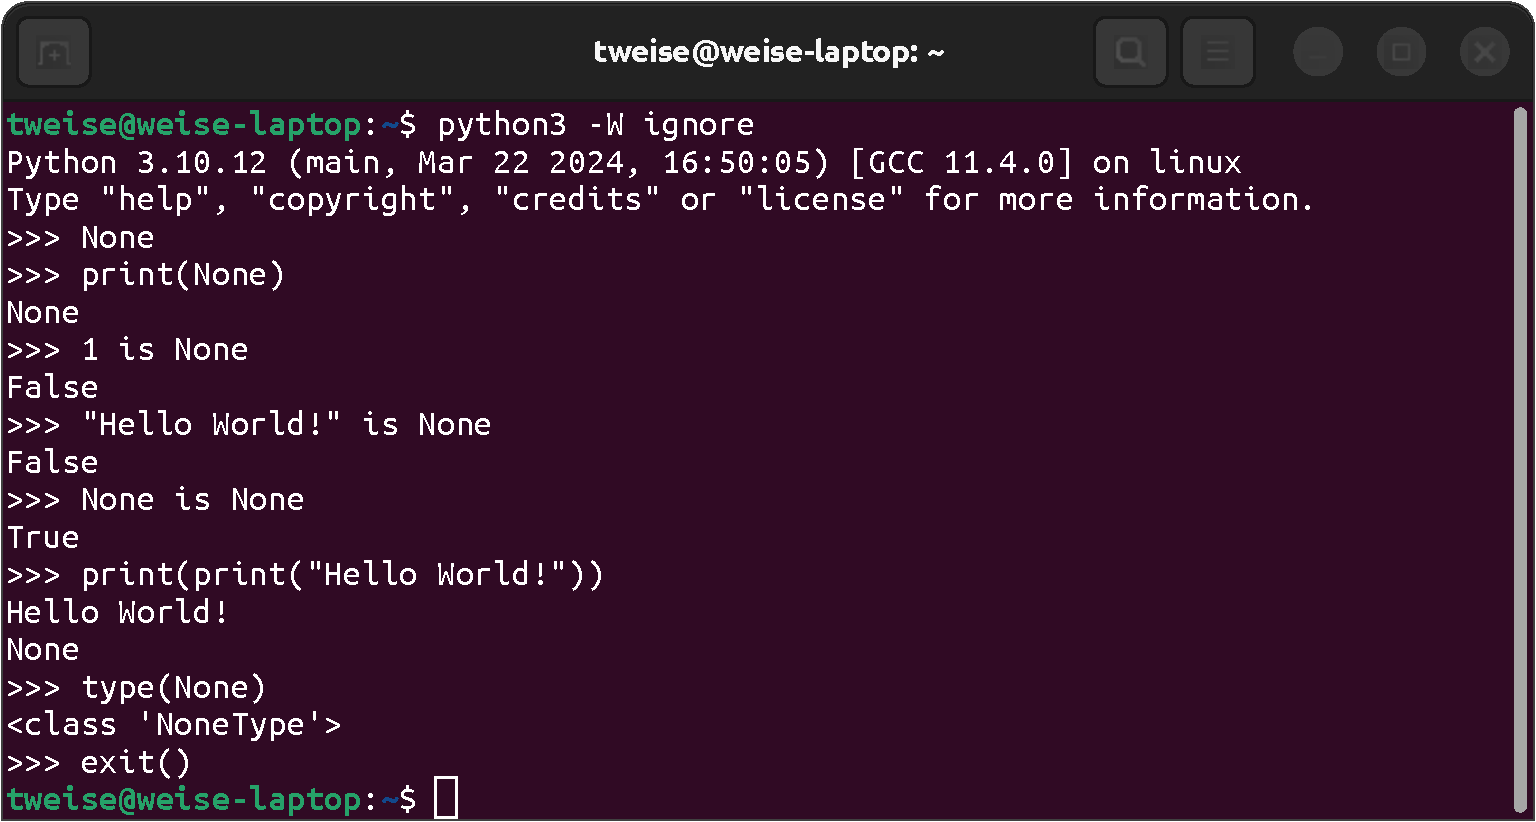
\includegraphics[width=0.7\linewidth]{\currentDir/none}%
\caption{Examples of using the value \pythonil{None}.}%
\label{fig:none}%
\end{figure}%
%
The last simple type we talk about is the \pythonilIdx{NoneType} and its one single value:~\pythonilIdx{None}.
Now you already learned the type \pythonil{bool} which can take on only two different values, \pythonil{True} and~\pythonil{False}.
You have also learned that the type \pythonil{float} has a special value called \inQuotes{Not a Number} and written as~\pythonilIdx{nan}.
So let's approach this new type from this direction.

\pythonilIdx{None} is used in scenarios where we want to specify that something does not have any value.
It is not an integer, float, string, or bool.
\pythonilIdx{None} is not equivalent to \pythonil{0}, it is not equivalent to~\pythonilIdx{nan}, and also different from the empty string~\pythonil{""}\pythonIdx{{\textquotedbl\textquotedbl}}.
It is just nothing.

\cref{fig:none} illustrates some of the things we can do with \pythonilIdx{None}.
If we write \pythonilIdx{None} into the \python\ console, then nothing happens.
In the past, we just wrote values, such as \pythonil{34} and, after we hit \keys{\enter}, they would be printed again.
Not so~\pythonilIdx{None}.
If we want to print~\pythonilIdx{None}, we have to force it by using the function \pythonilIdx{print}.
\pythonil{print(None)} then indeed prints~\pythonilIdx{None}.

The value \pythonilIdx{None} has many use cases.
Unfortunately, most of them we have not yet learned about, so we will have to circle back to this later.
For now, simply imagine that you want to write a program that step-by-step computes data.
Variables that have not yet been computed could be set to \pythonilIdx{None} to signify that.
If we had a \pythonil{float}, we could try to set it to \pythonil{nan} instead, but \pythonil{nan} could also be the result of a computation.
\pythonilIdx{None} would be much clearer, as no arithmetic calculation could ever return~\pythonilIdx{None}.

For this to work we need to be able to check whether a value is~\pythonilIdx{None}.
And we can do this using the operator~\pythonilIdx{is}.\footnote{%
\pythonilIdx{is} is a bit similar to \pythonilIdx{==}, but instead of comparing whether the contents of an object are the same, it compares whether two values reference the same object.}%
\pythonil{1 is None} gives us \pythonil{False} and so does \pythonil{"Hello World!" is None}.
\pythonil{None is None}, however, is \pythonil{True}.

Also, functions that do not return any result do, in fact, return~\pythonilIdx{None}.
We already learned some functions.
The function \pythonilIdx{len}, for example, can be used to compute the length of a string and then returns this value as~\pythonil{int}.
The function \pythonilIdx{log} from the \pythonilIdx{math} module computes the natural logarithm and returns a~\pythonil{float}.
\pythonilIdx{print}, however, just prints its parameter to the console {\dots} and returns \emph{nothing}.
Well, not \emph{nothing}.
It returns \pythonilIdx{None}!
We can test this by doing \pythonil{print(print("Hello World!))}.
The inner \pythonil{print("Hello World!)} will print the string~\pythonil{"Hello World!"}.
It will return~\pythonilIdx{None}.
This value \pythonilIdx{None} is then passed into the outer \pythonilIdx{print} function, which thus essentially does~\pythonil{print(None)} and, thus, prints \textil{None} to the console.
We therefore see two lines of text appear, first~\textil{Hello World} and then~\textil{None}.

The type of \pythonilIdx{None} can be determined using the \pythonilIdx{type} function and, indeed, is~\pythonilIdx{NoneType}.

A final use case for \pythonilIdx{None} is as default value for optional parameters of functions.
But we will learn this much later.
And thus, we conclude our short section about the value~\pythonilIdx{None} at this point.%
%
\endhsection%
%
